
\documentclass[t,8pt]{beamer}
\usepackage{amssymb}
\usepackage{amsfonts}
\usepackage{amsmath}
\usepackage{mathpazo}
\usepackage{hyperref}
\usepackage{multimedia}
\usepackage{comment}

\setcounter{MaxMatrixCols}{10}
\newenvironment{stepenumerate}{\begin{enumerate}[<+->]}{\end{enumerate}}
\newenvironment{stepitemize}{\begin{itemize}[<+->]}{\end{itemize} }
\newenvironment{stepenumeratewithalert}{\begin{enumerate}[<+-| alert@+>]}{\end{enumerate}}
\newenvironment{stepitemizewithalert}{\begin{itemize}[<+-| alert@+>]}{\end{itemize} }
\usetheme{AnnArbor}

\title[]{Quantile biomarkers based on single-cell multiplex immunofluorescence imaging data}

\author[]{{\large Inna Chervoneva, PhD}}

\institute{Professor\\ Division of Biostatistics\\
	     Department of Pharmacology, Physiology and Cancer Biology\\
	     Sidney Kimmel Medical College\\
	     \\Thomas Jefferson University, Philadelphia, PA}
\date{Pacific Symposium of Biocomputing (PSB), January 3, 2024}

\begin{document}

\frame{\titlepage}

	% % % % % % % % % % % % % % % % % % % % % % % % % % % % % % % % % % % % %  begin slide 5
	\frame
	{\frametitle{Breast cancer TMA data}   	   
		\begin{itemize}
			\item A tissue bank of invasive breast cancer (BC) tissue specimens from 1988-2012 was collected into core-based tissue microarrays (TMAs). 			
			\item Progression free survival up to 240 months follow-up for 1,000+ patients. 
			\item None of the patients received anti-cancer treatment prior to surgery
			\item The post-surgery treatments were captured by indicator variables for chemotherapy, radiation therapy, and hormone therapy. 
			\item The data also included commonly employed clinical-pathological prognostic factors: age, race (white vs. non-white), hormone receptor (HR) status, HER2 positivity, histologic grade, node status, tumor size ($<2 cm, 2-5 cm, >5cm$).
			\color{red}
			\item Immunofluorescence immunohistochemistry was performed for $\sim$100 proteins of interest
			\item Single-cell imaging data were generated for $\sim$25 proteins using the Definiens Tissue Studio software platform (Definiens AG).
		\end{itemize}
	           \begin{figure}
	    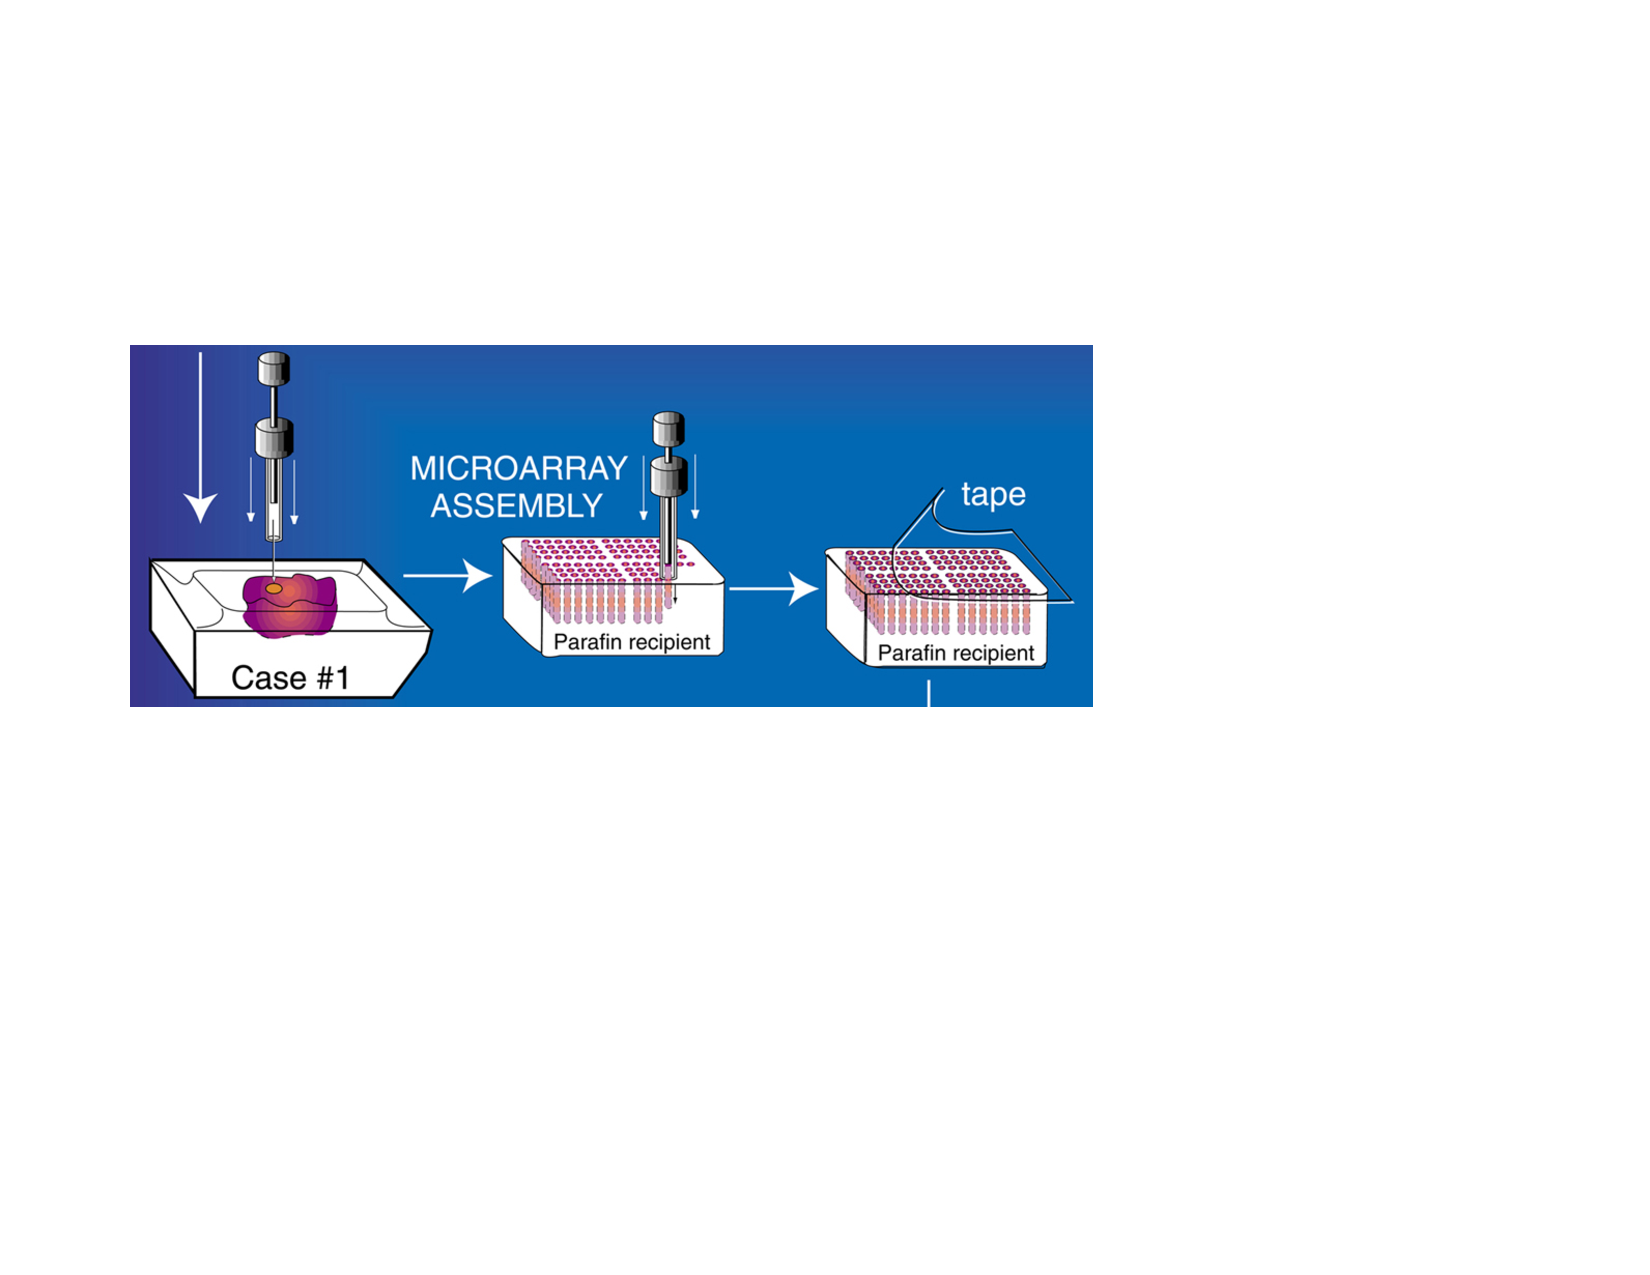
\includegraphics[width=3in]{Figures/TMA.pdf}
	   \end{figure} 			
	}

	% % % % % % % % % % % % % % % % % % % % % % % % % % % % % % % % % % % % %  begin slide 9
	\frame
	{\frametitle{Phosphorylated Stat5 (pYStat5) in breast cancer}   
		\begin{itemize}
			\item Representative Immunofluorescence immunohistochemistry images of human breast tissue 
			\item  pYStat5 (red), cytokeratin (green), and DAPI (blue).
                \item pYStat5 is a latent cytoplasmic transcription factor and a primary mediator of prolactin signaling in breast epithelia.
               \color{red}
                \item The loss of pYStat5 is a known risk factor for poor clinical outcome \cite{Peck11}
  		\end{itemize}              
	 \begin{figure}
                \includegraphics[width=4in] {/Users/ixc107/Documents/ICH_projects/grants/R01_ICH/QImethods/FRQIdata/Tran_pYStat5fig.pdf}
	\end{figure} 
	\begin{thebibliography}{ }
\begin{small}
\bibitem[Peck et al, 2011] {Peck11}
Peck, A. R., Witkiewicz, A. K., ... and Rui, H. (2011). 
Loss of nuclear localized and tyrosine phosphorylated Stat5 in breast cancer predicts poor clinical outcome and increased risk of antiestrogen therapy failure. Journal of clinical oncology, 29(18), 2448.
\end{small}
\end{thebibliography}	
	}
	
% % % % % % % % % % % % % % % % % % % % % % % % % % % % % % % % % % % % %  Types of markers
\frame
   {\frametitle{Functional vs. phenotypic single-cell protein biomarkers}  
   \begin{itemize} 
   	\item Information generated by the advanced quantitative pathology platforms include:		
	 \begin{itemize} 						
	      \item  \textbf{Cellular signal intensity (CSI)} of each protein expression in each compartment of interest (e.g. nucleus, membrane, cytoplasm of \textbf{every cancer cell}).
	      \item  The spatial coordinates of the cell centroids
	      \item Additional characteristics of the cells (area, shape factor, etc)
		\end{itemize}	
		    \color{red}  
 Single-cell protein biomarkers can be broadly classified as functional or phenotypic
  \color{black} 
        \item \textbf{Phenotypic markers} (identify cell types)
           \begin{itemize} 
             \item Cytokeratin
             \item “Cluster of differentiation” (CD) markers
             \item Other proteins characterizing immune or other stromal cells
           \end{itemize}           
   \item \textbf{Functional markers} (proteins of interest in potentially multiple cell types)
             \begin{itemize} 
              \item Proliferation markers (Ki-67, PCNA)
              \item Checkpoint proteins (PD-1, PD-L1, CTLA-4)
              \item Growth factors and receptors (EGFR, HER2, HER3)
         \end{itemize}               
   \item  Variety of spatial analysis approaches have been recently developed for phenotyped immune and cancer cells 
    \color{red}  
     \item Spatial analysis of quantitative functional markers is less explored and often proceeds with spatial analysis of "marker-positive" cells.                     
 \color{black}            
\end{itemize}
}


% % % % % % % % % % % % % % % % % % % % % % % % % % % % % % % % % % % % % Marked point processes approach
	\frame
	{\frametitle {Marked point processes framework for analysis of single-cell protein data}  
		\begin{itemize} 
		   \item The point patterns of cell centroids are viewed as realizations of a point process.
			\item A \textbf{marked point pattern} is a point pattern combined with (`marks') measured at each cell.	
			 \item Point pattern of cell centroids  + continuous measures of CSI levels of protein expression \\ $=>$ \textbf{marked point pattern (MPP)}		
			\item Categorical marks capturing cell phenotypes combined with point pattern of cell centroids $=>$  \textbf{multitype marked point pattern (MMPP)}.
               		\color{blue}
		  \item  \textbf{If marks values are independent from their spatial locations, then it is sufficient to consider marginal distribution of marks irrespective of the point locations!}
		\end{itemize} 
  \begin{columns}[T]
		      \begin{column}{0.6\textwidth}		      
			 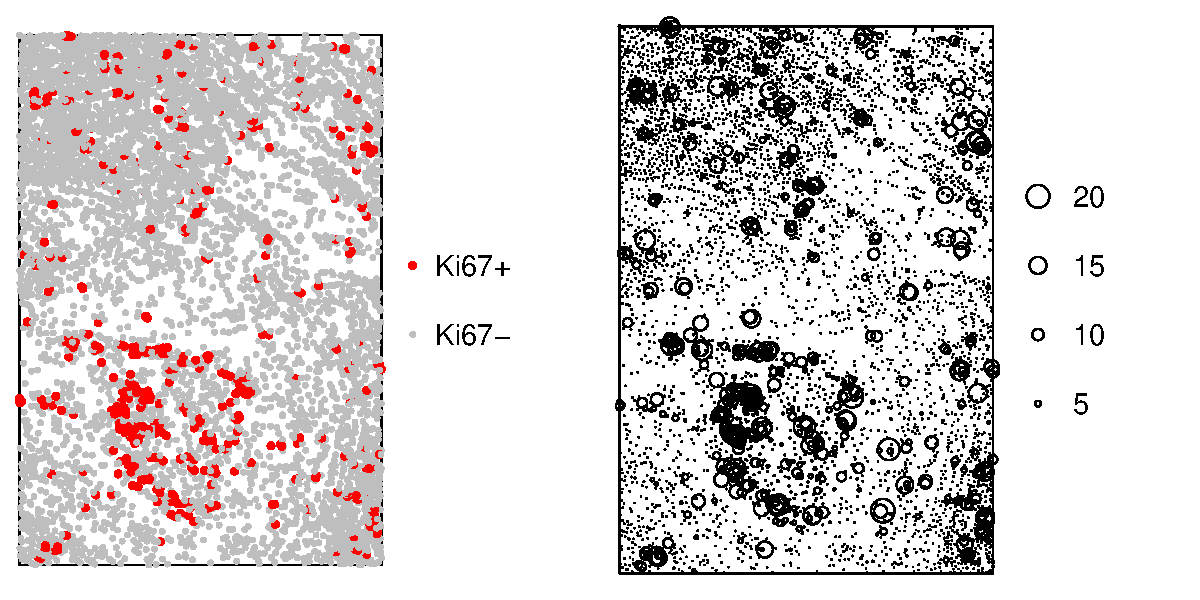
\includegraphics[height=1.45in] {Figures/Ki67both.pdf}
			 Ki67 is protein associated with cellular proliferation
		      \end{column}
		\begin{column}{0.35\textwidth}
		 E.g. independence between Ki67 CSI levels and cancer cell locations was evaluated in 1958 TMA cores\\
		 % using the test statistics based on conditional mean (Emark), conditional variance (Vmark), and mark correlation (markcorr)
		\color{red}
	  	 \textbf{The null hypothesis of independence between marks and points was rejected in $27-39\%$ of TMA cores}
		   \color{black}
		   (somewhat different results using conditional mean, conditional variance or mark correlation)	
		\end{column}		
	\end{columns}
	}

% % % % % % % % % % % % % % % % % % % % % % % % % % % % % % % % % % % % %  	
%\frame
%   {\frametitle{Spatial vs. marginal distribution analysis of MPPs}  
%}


	
		% % % % % % % % % % % % % % % % % % % % % % % % % % % % % % % % % % % % % slide 10
	\frame
	{\frametitle{Sample distributions of pYStat5 CSI levels}   
\begin{itemize}
	\item The standard approach for analysis of functional biomarkers: \textbf{Mean Signal Intensity (MSI)} is computed within the region
of interest (i.e. cancer cell compartment of the tumor).
		 \color{red}	
                   \item But the same MSI levels  may correspond to different CSI distributions. 
       		\color{black}	
          \end{itemize}  

  \begin{columns}[T]
		      \begin{column}{0.65\textwidth}
			\includegraphics[width=3.2in] {/Users/ixc107/Documents/ICH_projects/grants/R01_ICH/presentations/JSM2021/mock_Density_fig.pdf}
		      \end{column}
		\begin{column}{0.3\textwidth}
		\begin{itemize}
		  \item distribution of Log CSIs in two sample tissues
              	  \item  blue lines show the kernel density estimates 
	  	   \item  black vertical lines show the MSIs
             \end{itemize}  
		\end{column}		
	\end{columns}
\begin{itemize}
 \color{red}
	\item Distributions of CSI levels may be represented with densities or \textbf{quantile functions}
  \color{black}		
          \end{itemize}  		
	 
	  \begin{columns}[T]
		\begin{column}{0.65\textwidth}
			 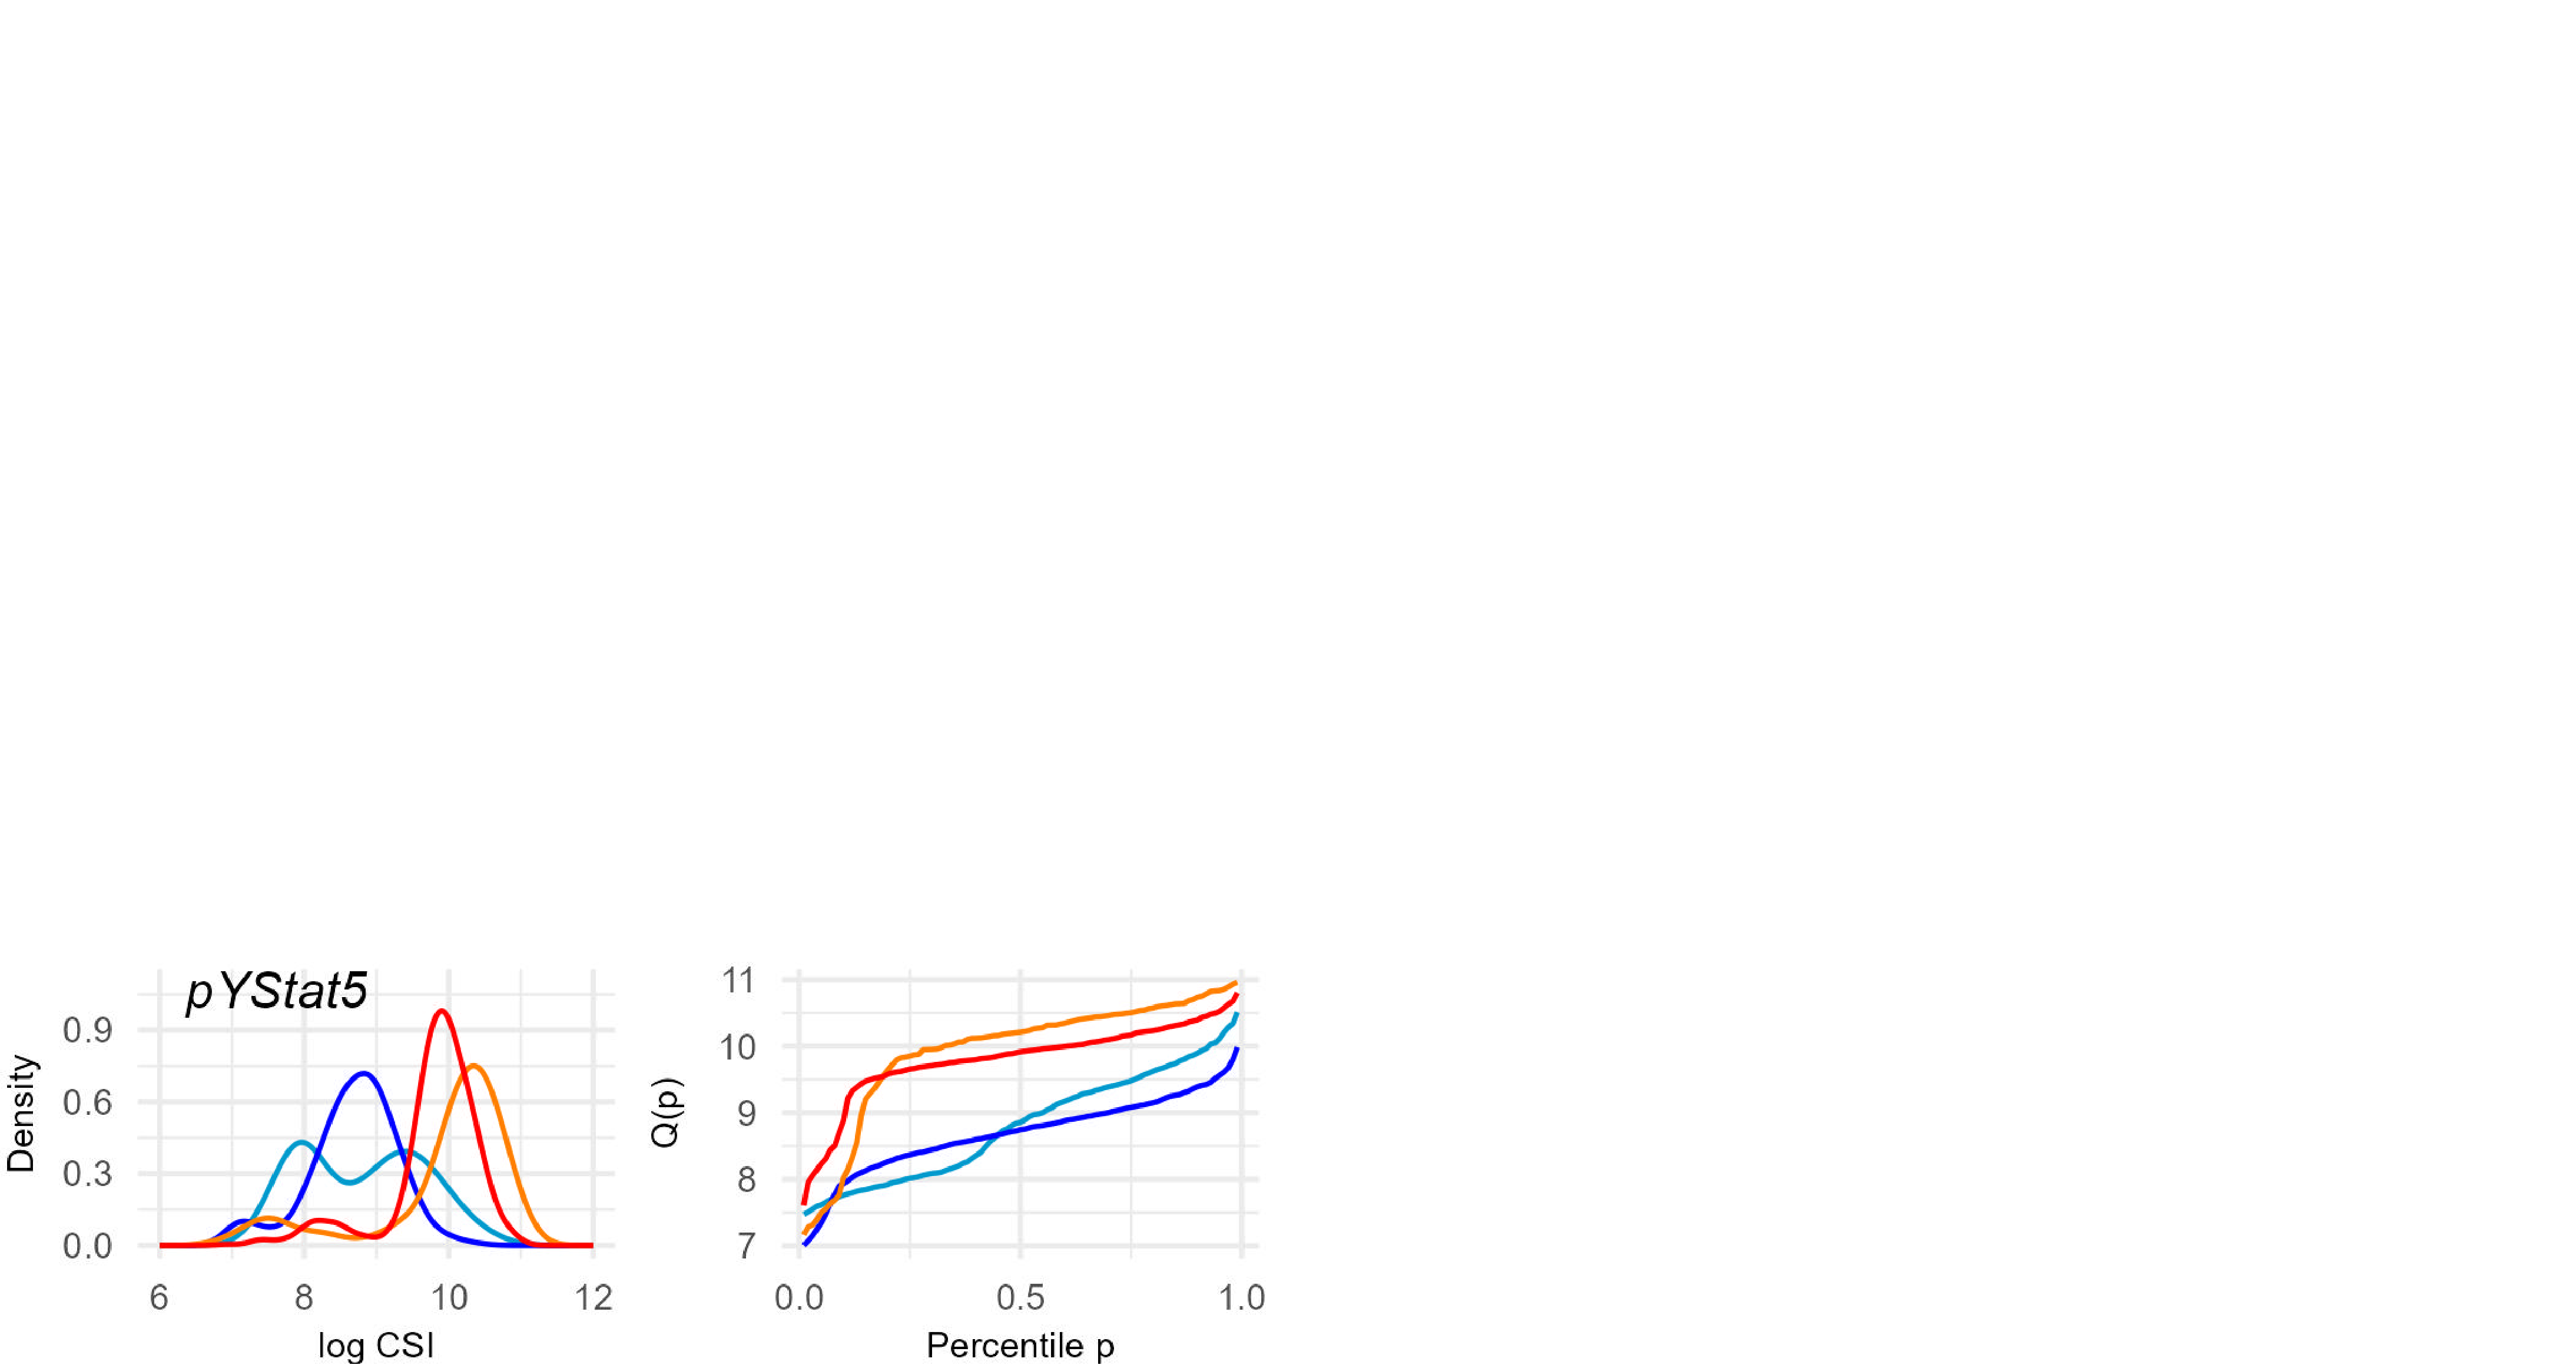
\includegraphics[width=3.2in] {Figures/densities_quantiles.pdf}
		\end{column}
		
		\begin{column}{0.3\textwidth}
		\begin{itemize}
              	  \item Lines of the same color show the kernel density estimate and the sample quantile function for pYStat5 CSI levels in the same sample tissue
             \end{itemize}  
		\end{column}
	\end{columns}			
		
	}
	
	% % % % % % % % % % % % % % % % % % % % % % % % % % % % % % % % % % % % % begin slide  12	
	
	\frame
	{\frametitle{Functional Regression Quantile Index (FR-QI)}
		\begin{itemize}	
		    \item  For $k^{th}$ subject, let the  \color{red} empirical quantile function $Q_{k}(p)$  \color{black} of CSI expressions
         be defined as the $j^{th}$ order statistic, where $j$ is such that $(j-1)/n<p<j/n$. 	
		\item   \color{red} \textbf{FR-QI}  \color{black} is defined as the functional regression  \cite{James02} predictor,
			 \color{red}
		 \begin{center}
		 	$QI_{k}= \int_{0}^{1} \beta(p)Q_{k}(p)dp$
		\end{center}
			 \color{black}
		\linebreak
		where $\beta(p)$ is an unknown functional coefficient function  \cite{Yi23}
\item $\beta(p)$ is represented by a spline or by a piece-wise linear function and estimated as part of fitting a model to a data set that includes clinical outcomes. 
	\item For continuous or categorical outcomes, $\beta(p)$ may be estimated using the R package \texttt{refund} or using the \texttt{gam} function in the R package \texttt{mgcv}  
	\item For survival outcomes, $\beta(p)$ is estimated by flitting a proportional hazard functional regression model \cite{Gellar15}, a.k.a. Linear Functional Cox Model (LFCM):
              \begin{center}
		 	$log h_{k}(t, \beta())=log h_{0} (t)+ \int_{0}^{1} \beta(p)Q_{k}(p)dp$
	    \end{center}
where $h_{k}[t|\beta, Q_{k}]$ is the hazard function for the $k^{th}$ subject at time $t$ and $h_{0}(t)$ is a non-parametric baseline hazard function.		     
 \item LFCM can be fitted using the \texttt{gam} function in the R package \texttt{mgcv}   
		\end{itemize}
\begin{thebibliography}{ }
\begin{footnotesize}
\bibitem[James, 2002] {James02}
James G. Generalized linear models with functional predictor variables. \textit{Journal of the Royal Statistical Society}. 2002; 64(Series B):411-32.	
\bibitem[Yi et al, 2023a] {Yi23}
Yi, M., Zhan, T., Peck, A. R., Hooke, J. A., Kovatich, A. J., Shriver, C. D., ... & Chervoneva, I. (2023a). Quantile Index Biomarkers Based on Single-Cell Expression Data. Laboratory Investigation, 103(8), 100158.
\bibitem[Gellar et al, 2015] {Gellar15}
Gellar, J. E., Colantuoni, E., Needham, D. M., and Crainiceanu, C. M. (2015), “Cox Regression Models With Functional Covariates for Survival Data,\textit{Statistical Modelling}, 15, 256–278.
\end{footnotesize}
\end{thebibliography}			

}		

	
% % % % % % % % % % % % % % % % % % % % % % % % % % % % % % % % % % % % % begin slide  13
	\frame
	{\frametitle{Illustration of computing FR-QI}
		\begin{figure}
                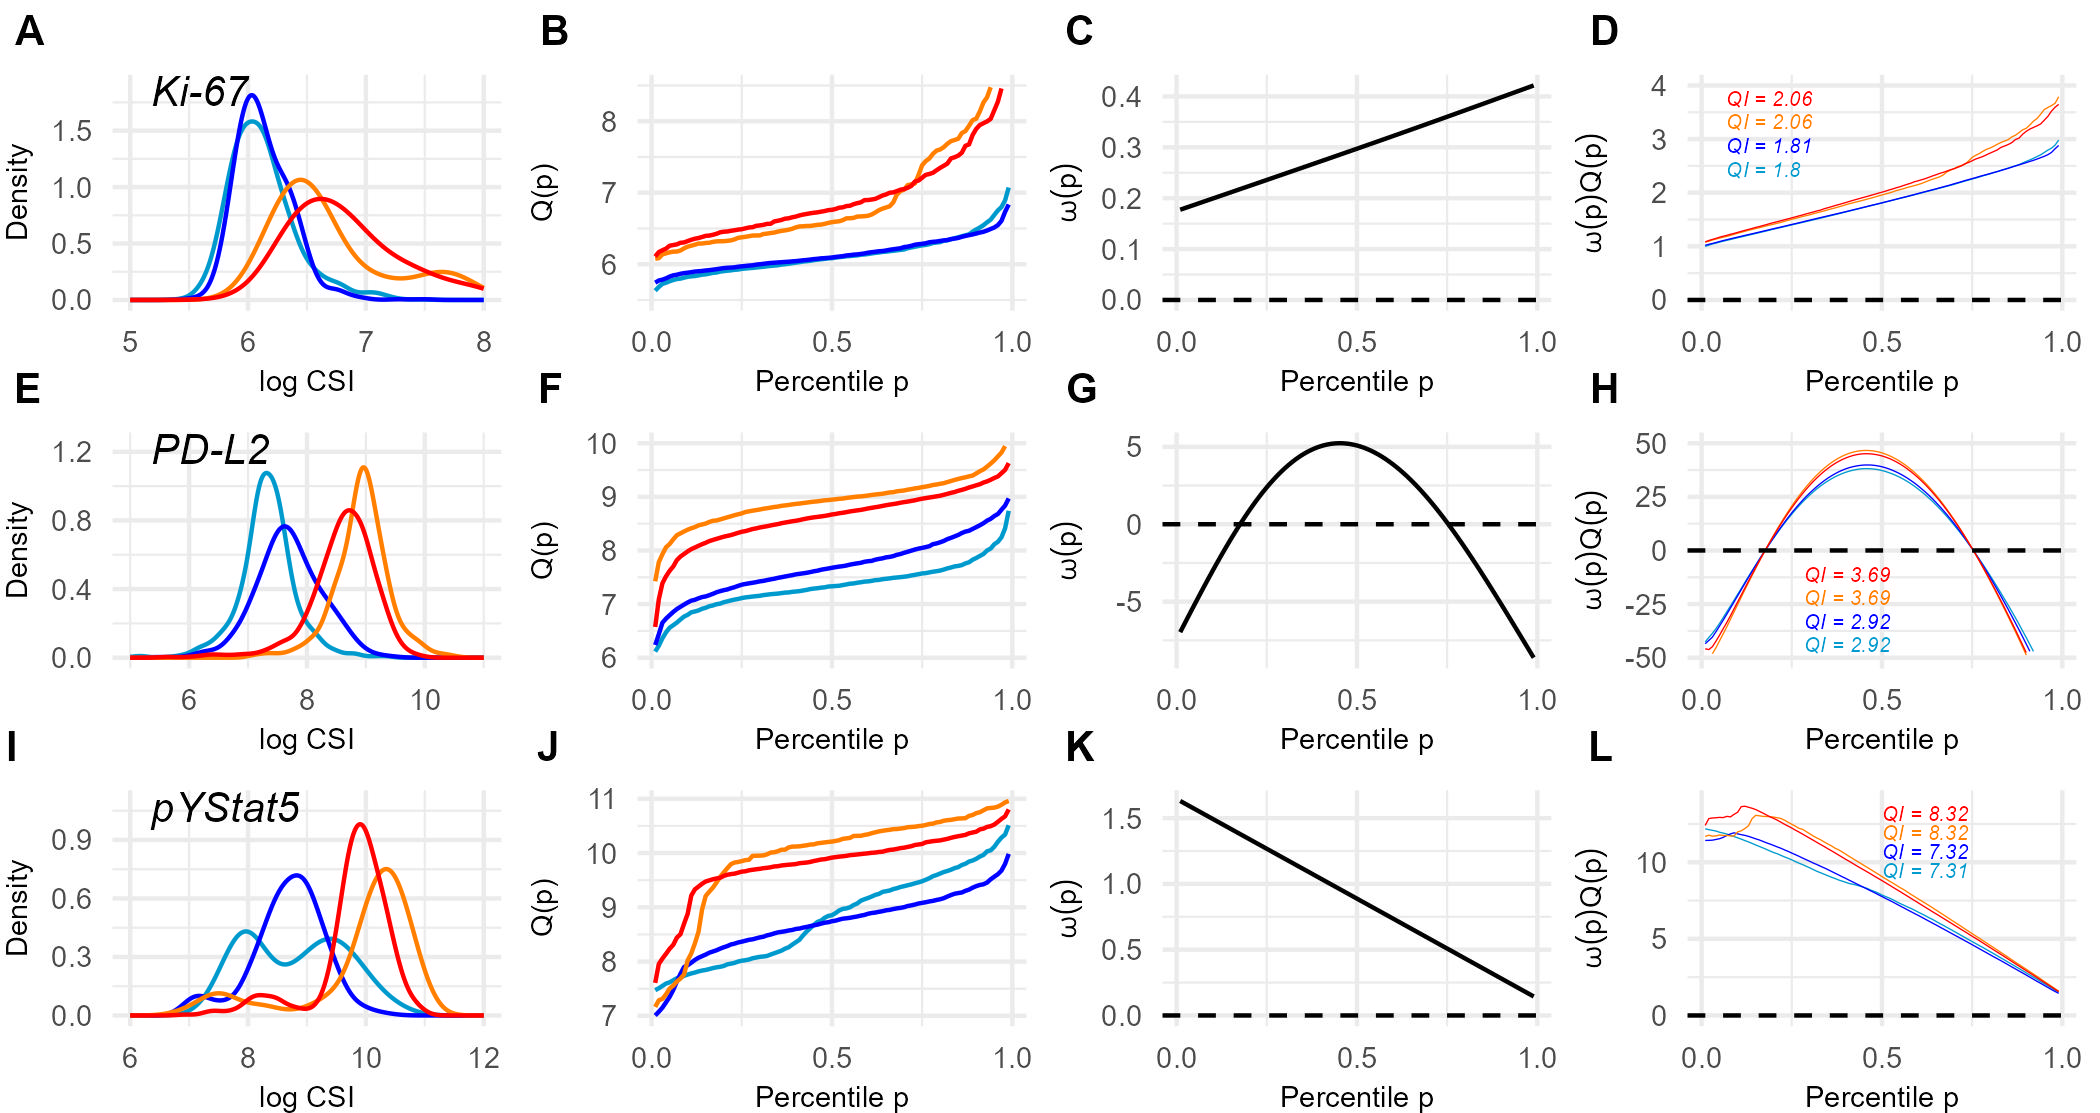
\includegraphics[width=4.8in] {Figures/computingFRQI.jpeg}
		\end{figure} 
	}

% % % % % % % % % % % % % % % % % % % % % % % % % % % % % % % % % % % % %  	nlFR-QI

\frame
   {\frametitle{Nonlinear Functional Regression Quantile Index (nlFR-QI)}
   \begin{itemize}	
%\color{red}
    \item \textbf{nlFR-QI} is defined as a nonlinear functional regression predictor,
    			 \color{red}
		 \begin{center}
		 	nlFR-QI$_{k}= \int_{0}^{1} F(p, Q_{k}(p))dp$
		\end{center}
where F(·,·) is an unspecified bivariate twice differentiable function. 
		  \color{black}
  \item F(·,·) is represented by a tensor product of univariate P-splines \cite{McLean}
              \begin{center}
		 	$F(s,x)=\sum^{N_s}_{i=1} \sum^{N_x}_{l=1} \theta_{i,l} B_{i}(s) B_{l}(x)$
	     \end{center}
where $B_{i}$ and $B_{l}$ are univariate splines on the domains of $s$ and $x$, respectively.	    	
    \item  Then \textbf{nlFR-QI}$_{k}$ can be re-written as
               \begin{center}
$\int_{0}^{1} \sum^{N_s}_{i=1} \sum^{N_x}_{l=1} \theta_{i,l} B_{i}(p) B_{l}(Q_{k}(p)) dp = 
\sum^{N_s}_{i=1} \sum^{N_x}_{l=1} \theta_{i,l} \int_{0}^{1} B_{i}(p) B_{l}(Q_{k}(p))dp=$\mathbf{V}^T_{k}\boldsymbol{\theta}$
	     \end{center}		
	\item For survival outcomes, F(·,·) is estimated by fitting an Additive Functional Cox Model (AFCM) \cite{Cui20} 
	   \begin{center}
		 	$log h_{k}(t, F, Q_{k})=log h_{0} (t)+ \int_{0}^{1} F(p, Q_{k}(p))dp$
	    \end{center}
maximizing the penalized partial log-likelihood using \texttt{gam} function in the R package \texttt{mgcv}.
\item The \texttt{gam} function may be also used with continuous or categorical outcomes
 \item Identifiability constraints are imposed by default in R mgcv package.
       
\end{itemize}
\begin{thebibliography}{ }
\begin{footnotesize}
\bibitem[Cui et al, 2020] {Cui20}
Cui, E., Crainiceanu, C.M. and Leroux, A., 2020. Additive Functional Cox Model. Journal of Computational and Graphical Statistics, pp.1-14.
\bibitem[McLean et al, 2014] {McLean}
McLean, M. W., Hooker, G., Staicu, A.-M., Scheipl, F., and Ruppert, D. (2014), “Functional Generalized Additive Models,” Journal of Computational
and Graphical Statistics, 23, 249–269.
\end{footnotesize}
\end{thebibliography}			
}

% % % % % % % % % % % % % % % % % % % % % % % % % % % % % % % % % % % % %  	
\frame
   {\frametitle{Estimated F(·,·) surfaces for nlFR-QIs as predictors of PFS}  
   \begin{itemize}	
	\item Estimated surface from AFCM using  \color{red}  \textbf{pYStat5}  \color{black} CSI quantile function
	\end{itemize}		
	  \begin{columns}[T]
		\begin{column}{0.6\textwidth}
			 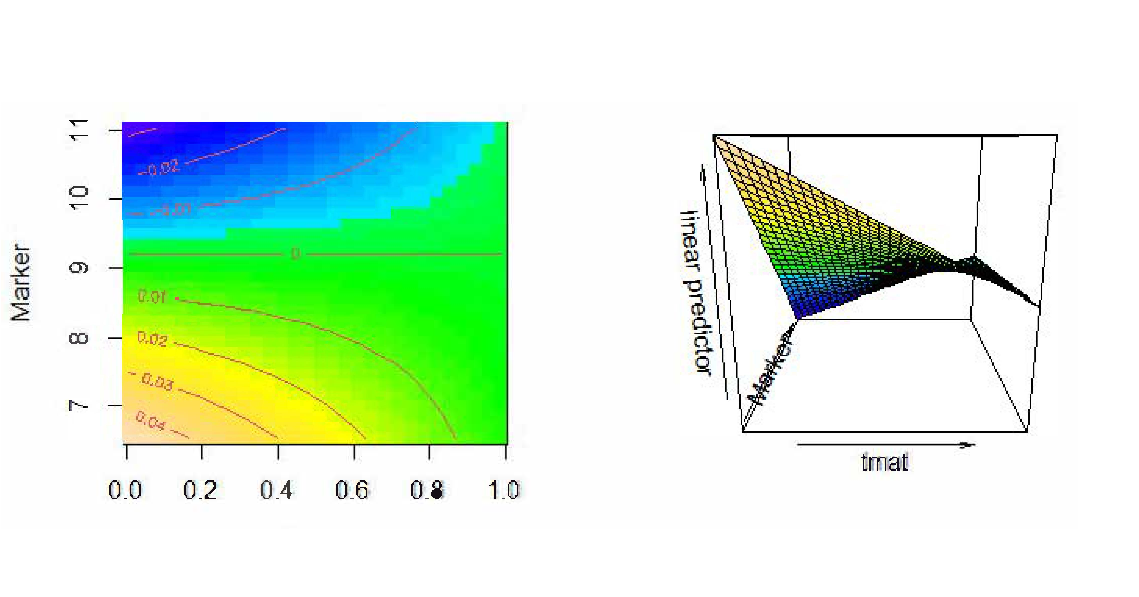
\includegraphics[width=3in] {Figures/pYStat5_afcm.pdf}
		\end{column}	
		\begin{column}{0.3\textwidth}
              	 \color{red}  \textbf{pYStat5}  \color{black} $Q(p)$ function\\
	         \begin{itemize}
                  \item as linear functional regression
	          predictor in LFCM: $p < 0.001$
		 \item as nonlinear functional regression
			predictor in AFCM: $p < 0.001$
             \end{itemize}  
		\end{column}
	\end{columns}		
   \begin{itemize}	
	\item Estimated surface from AFCM using  \color{red}  \textbf{PR}   \color{black} CSI quantile function
	\end{itemize}			
	  \begin{columns}[T]
		\begin{column}{0.6\textwidth}
	 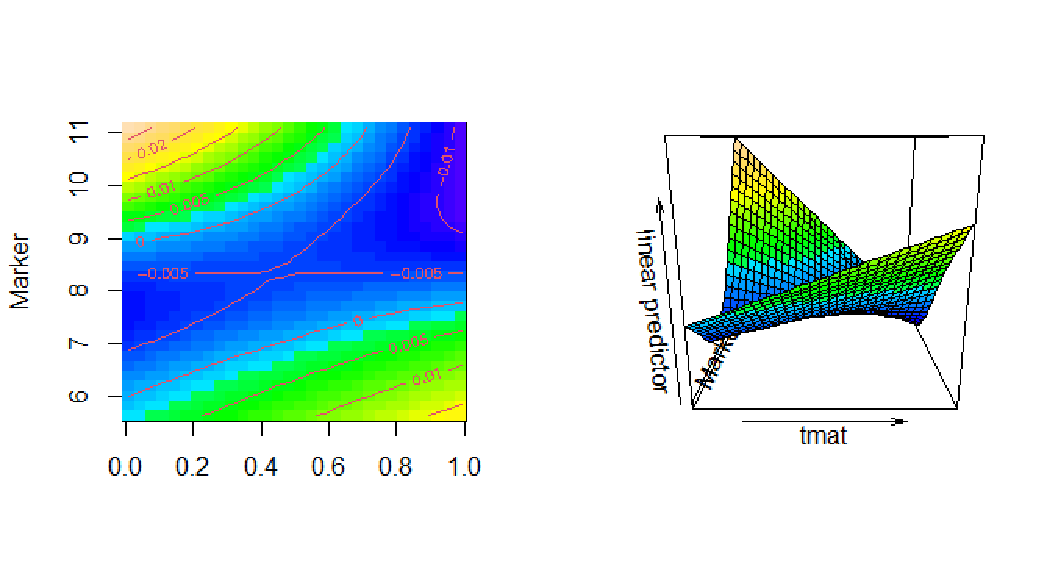
\includegraphics[width=3in] {Figures/PR_afcm.pdf}
		\end{column}	
		\begin{column}{0.3\textwidth}
		 \color{red}  \textbf{PR}   \color{black} $Q(p)$ function\\
		\begin{itemize}
	             \item as linear functional regression
	             predictor in LFCM: $p=0.039$
		        \item  as nonlinear functional regression
			predictor in AFCM: $p=0.007$
             \end{itemize}  
		\end{column}
	\end{columns}		
	      
}

% % % % % % % % % % % % % % % % % % % % % % % % % % % % % % % % % % % % %  	
\frame
   {\frametitle{Effects of FR-QI and nlFR-QI in the external validation cohort}  
      \begin{itemize}
        \item The external validation cohort includes 273 ER+ patients with 31 progression events
        \item Results for Ki67, PD-L2, and Ki67 FR-QIs are reported in \cite{Yi23}
          \end{itemize}
		\begin{figure}
                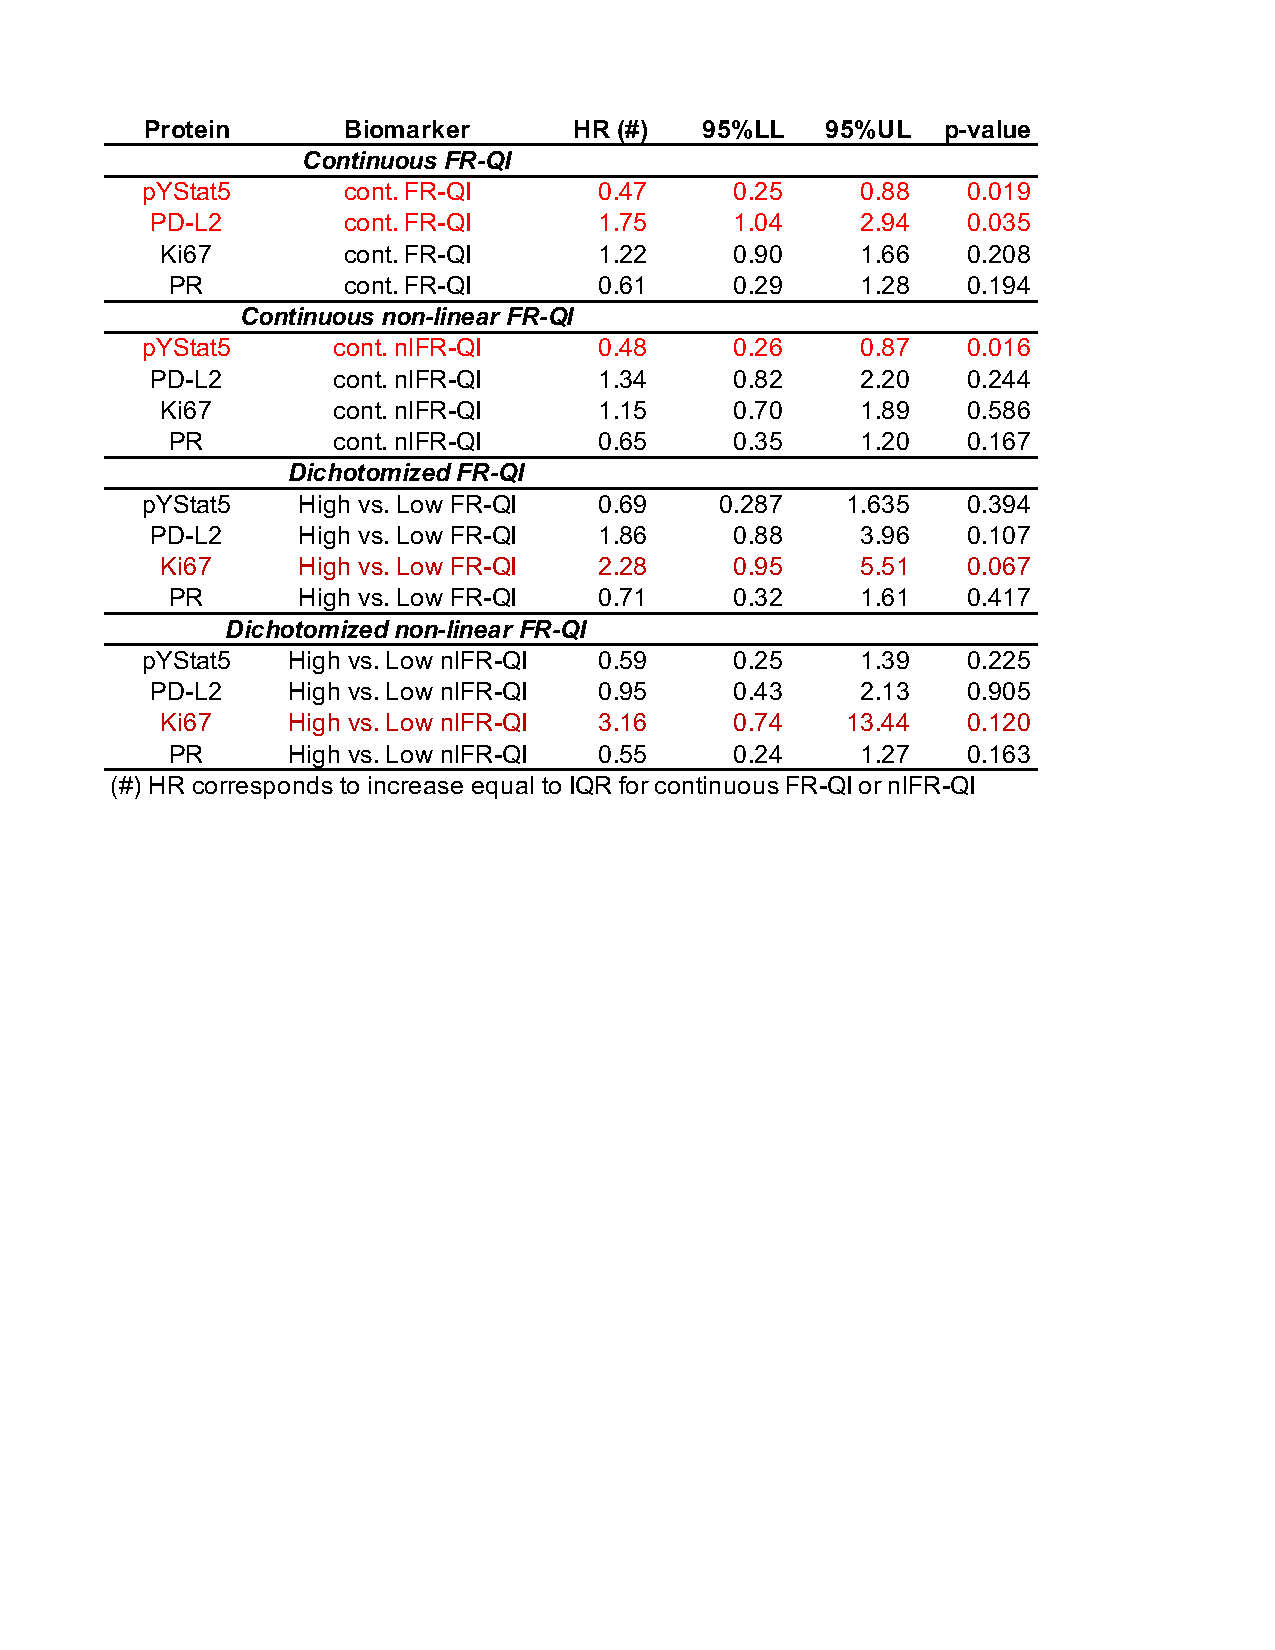
\includegraphics[width=2.8in] {Figures/Tables.pdf}
		\end{figure} 
\begin{thebibliography}{ }
\begin{footnotesize}
\bibitem[Yi et al, 2023a] {Yi23}
Yi, M., Zhan, T., Peck, A. R., Hooke, J. A., Kovatich, A. J., Shriver, C. D., ... & Chervoneva, I. (2023a). Quantile Index Biomarkers Based on Single-Cell Expression Data. Laboratory Investigation, 103(8), 100158.
\end{footnotesize}
\end{thebibliography}
}


% % % % % % % % % % % % % % % % % % % % % % % % % % % % % % % % % % % % %  	
\frame
   {\frametitle{R package \texttt{Qindex} for computing FR-QI and nlFR-QI}
   
   \begin{itemize}	
	\item  R package \texttt{Qindex} implements FR-QI and nlFR-QI 
	\item  \texttt{Qindex} is available in the CRAN depository https://CRAN.R-project.org/package=Qindex.
     \item Function \texttt{FRindex} in the package \texttt{Qindex} can be used to estimate $\beta$ in the training data set and compute FR-QI for each subject in the training and a new test data set, if available.
          \item Function \texttt{nlFRindex} in the package \texttt{Qindex} can be used to estimate $F(·,·)$ in the training data set and compute nlFR-QI for each subject in the training and a new test data set, if available.
     \item FR-QI methodology and implementation in \texttt{Qindex} is described in \cite{Yi23}      	       
    \item Additional functions in package \texttt{Qindex} 
         \begin{itemize}
    \item facilitate computations of sample quantiles in each cluster of observations
   (function \texttt{clusterQp})
  \item  identify optimal dichotomized continuous predictors using repeated split sampling
  (function \texttt{optimSplit$\textunderscore$dichotom})
   \item  compute bootstrap-based optimism correction for testing optimally dichotomized predictors in multivariable models
   (function \texttt{BBC$\textunderscore$dichotom})
     \end{itemize}
   \item R package \texttt{Qindex} also implements Optimal Quantile biomarkers described in \cite{Yi23BMC}       
  \end{itemize}
\begin{thebibliography}{ }	
\begin{small}
\bibitem[Yi et al, 2023a] {Yi23}
Yi, M., Zhan, T., Peck, A. R., Hooke, J. A., Kovatich, A. J., Shriver, C. D., ..., Chervoneva, I. (2023a). Quantile Index Biomarkers Based on Single-Cell Expression Data. Laboratory Investigation, 103(8), 100158.
\bibitem[Yi et al, 2023b] {Yi23BMC}
Yi, M., Zhan, T., Peck, A. R., Hooke, J. A., Kovatich, A. J., Shriver, C. D., ... & Chervoneva, I. (2023b). Selection of optimal quantile protein biomarkers based on cell-level immunohistochemistry data. BMC bioinformatics, 24(1), 298.
\end{small}
\end{thebibliography}	

}


% % % % % % % % % % % % % % % % % % % % % % % % % % % % % % % % % % % % %  	
\frame
   {\frametitle{Optimal quantile biomarkers \cite{Yi23BMC}}  
Algorithm to identify the optimal $Q(p)$ predictor of an outcome in a screening data set:\\
	 \begin{itemize} 
	\item Select the set of quantiles to be evaluated as predictors.\\
	\item  For each random split into training/test set pair and each considered quantile, \\
		 \begin{itemize} 
   \item Determine the optimal cutoff (e.g. using the R package rpart) in the training set. \\
  \item  Apply the optimal cutoff to the test set and estimate the effect size (e.g. log odds ratio).\\
   	 \end{itemize} 
  \item  Repeat for 100 training/test splits, compute the median effect size for each quantile.\\
  \item  Select the optimal quantile with the highest effect size. \\
  \item Perform bootstrap-based optimism correction if there are no external validation data. 
   	 \end{itemize} 
\bigskip

\textbf{Screening cohort}: 845 non-metastatic hormone positive (HR+)
breast cancer patients with 142 progressions and the clinical follow-up ranging from
2 months to 238 months with median follow-up time of 115 months.

\textbf{External validation cohort}: 340 non-metastatic HR+ breast cancer patients with 42
progression events and clinical follow-up ranging from 0.8 months to 297.5 months with a median follow-up time of 148 months.

\bigskip
\begin{thebibliography}{ }	
\begin{small}
\bibitem[Yi et al, 2023b] {Yi23BMC}
Yi, M., Zhan, T., Peck, A. R., Hooke, J. A., Kovatich, A. J., Shriver, C. D., ... & Chervoneva, I. (2023b). Selection of optimal quantile protein biomarkers based on cell-level immunohistochemistry data. BMC bioinformatics, 24(1), 298.
\end{small}
\end{thebibliography}
}

% % % % % % % % % % % % % % % % % % % % % % % % % % % % % % % % % % % % %  	
\frame
   {\frametitle{Results from \cite{Yi23BMC}}  

\begin{figure}
                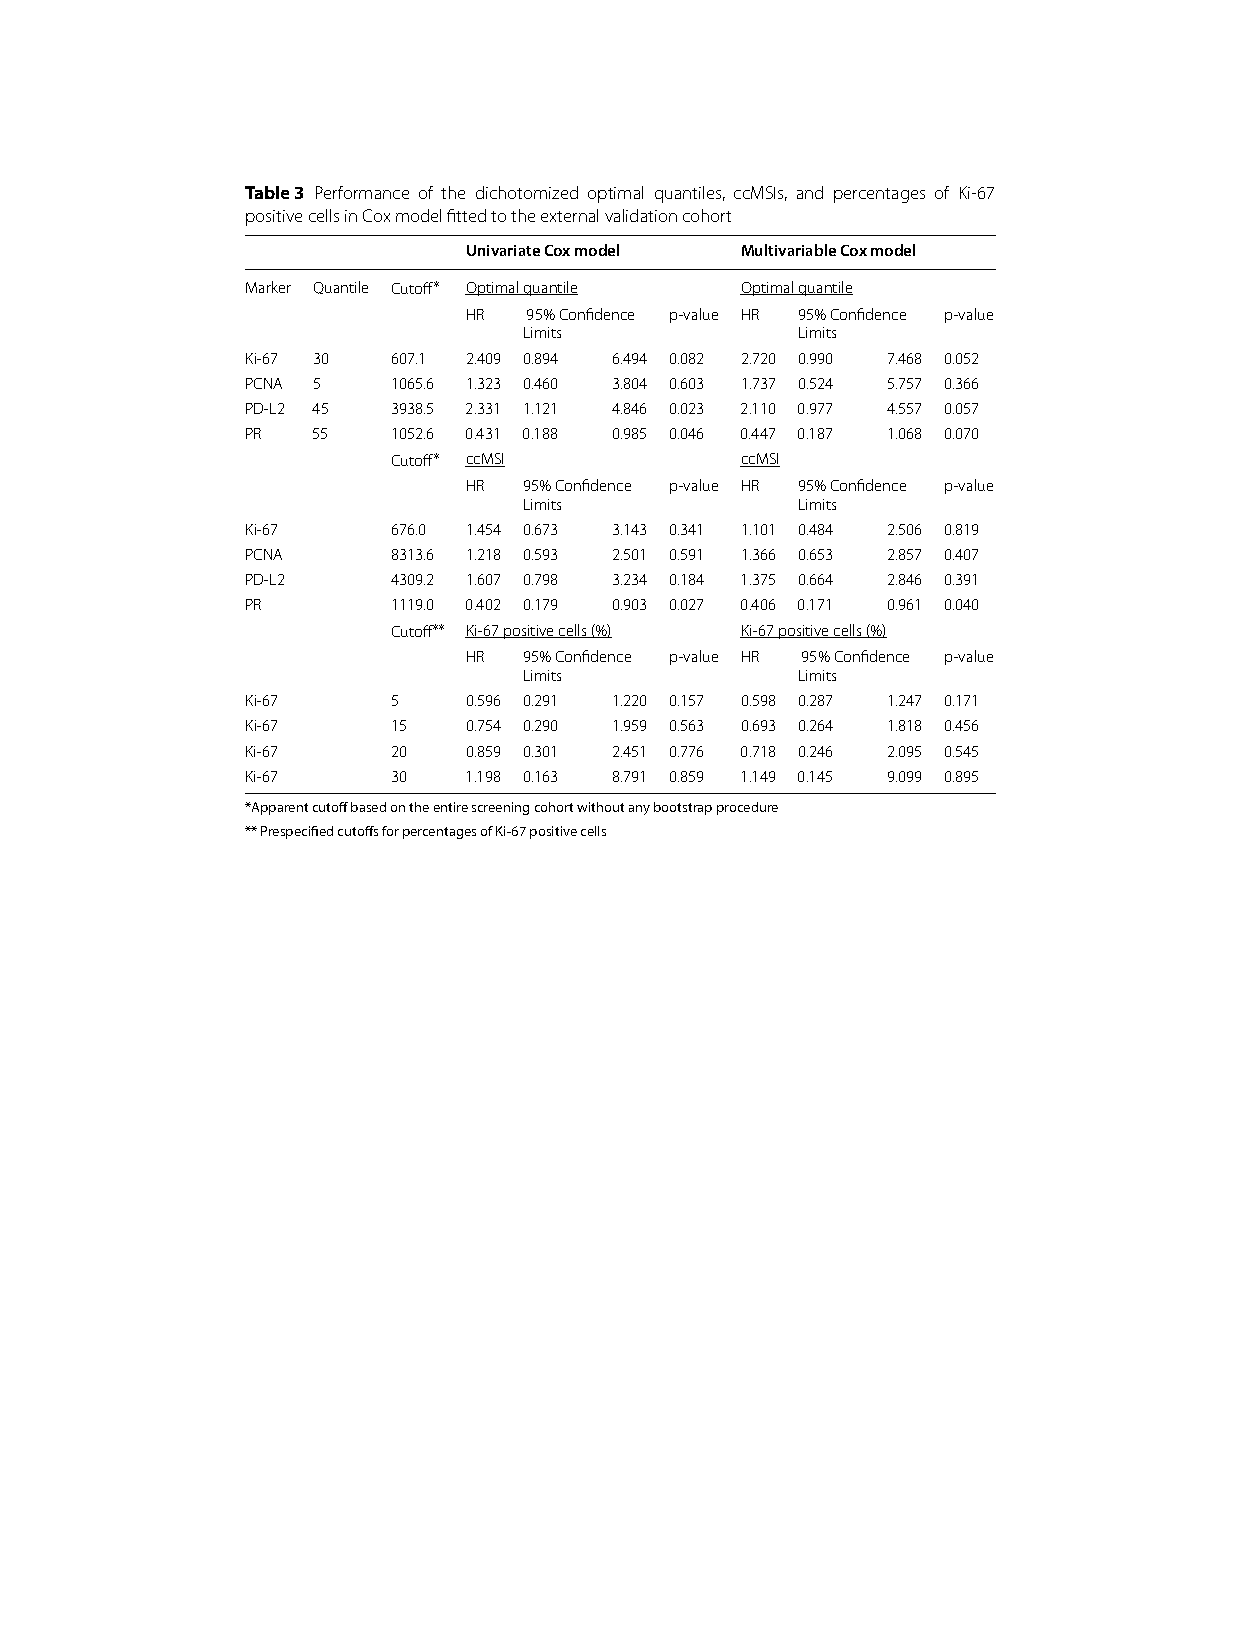
\includegraphics[width=3.5in] {Figures/Yi_et_al_BMC_Bioinf_2023.pdf}
 \end{figure} 

}

% % % % % % % % % % % % % % % % % % % % % % % % % % % % % % % % % % % % %  	
\frame
   {\frametitle{Design of the simulation studies}  	 
     \begin{columns}[T]
		      \begin{column}{0.4\textwidth}
			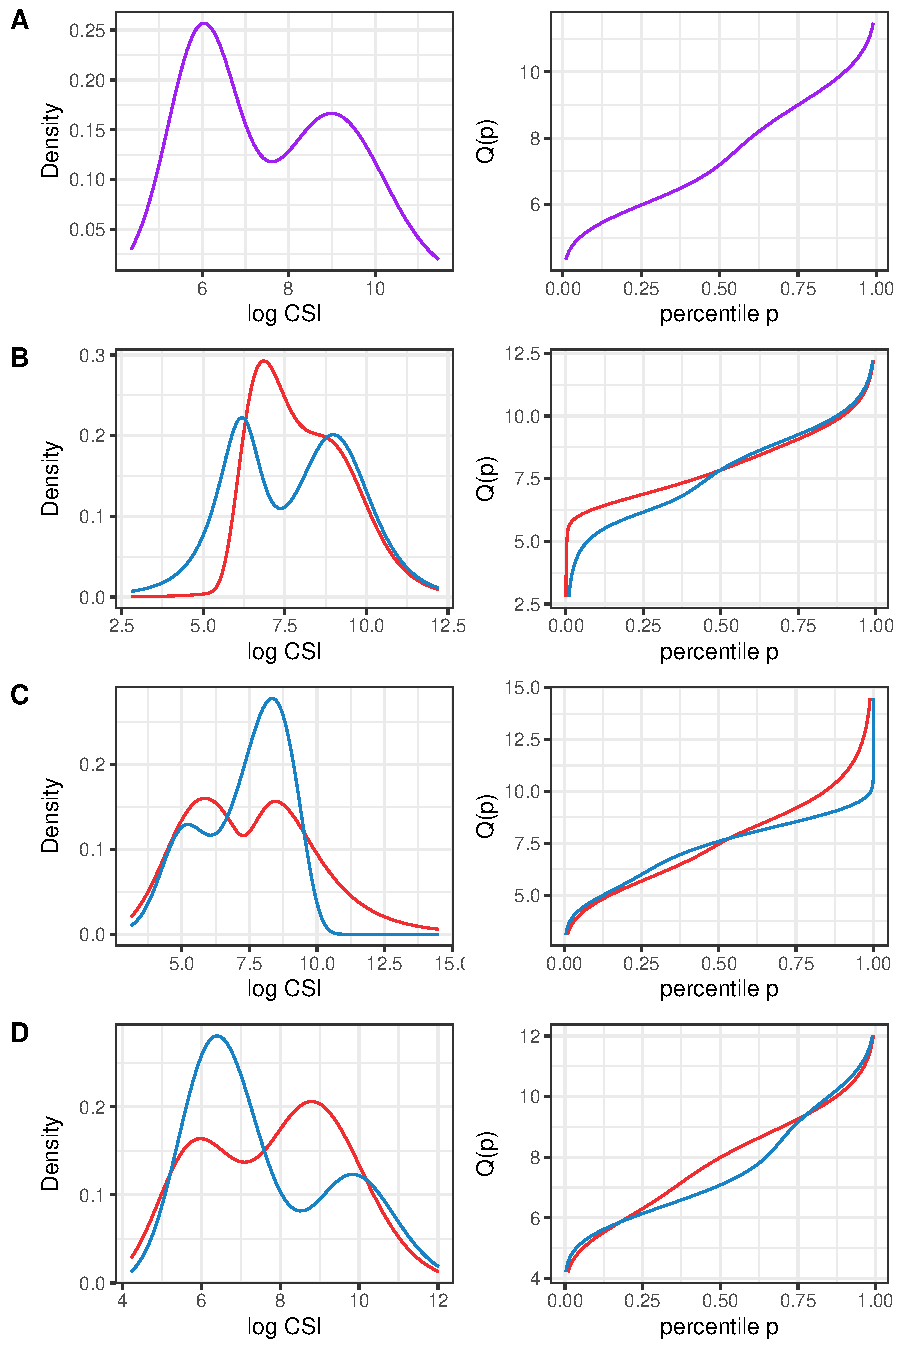
\includegraphics[width=2in] {Figures/Figures_simulations/density.quantile.plot.pdf}
		      \end{column}
		\begin{column}{0.6\textwidth}
	   	\begin{itemize} 
	\item Survival times were generated using the R package \texttt{survsim}  \cite{survsim}
	\item Each simulated data set included high-risk and low-risk groups such that the hazard ratio associated with high-risk group ranged in (i) [2,3] or (ii) [3,4].
		\item CSIs per subject: N = 20, 100, 200, 500, 1000. 
	\item Distributions of CSI values were simulated as mixtures of two 4-parameter Tukey's $g$-\&-$h$ distributions using the R package \texttt{QuantileGH} 
	\item For scenario A, low- and high-risk groups had the same CSI distribution.  For scenarios B,C,D, simulated CSI densities are shown as blue curves for low-risk group
	 and as red curves for high-risk group.
	\item FR-QI biomarkers were based on a small (19) or a large (99) number of percentiles.
	\item 1000 pairs of training and test sets with 120 subjects per risk group were simulated per each scenario.
  \end{itemize}   	
\begin{thebibliography}{ }	
\begin{footnotesize}
\bibitem[Morina and Navarro, 2014] {survsim}
Morina, D. and Navarro, A., 2014. The R package survsim for the simulation of simple and complex survival data. Journal of Statistical Software, 59, pp.1-20.
\end{footnotesize}
\end{thebibliography}	
		      \end{column}		
	\end{columns} 
}

	% % % % % % % % % % % % % % % % % % % % % % % % % % % % % % % % % % % % %  	
\frame
   {\frametitle{Mixtures of Tukey's $g$-\&-$h$ distributions }  

Tukey's $g$-\&-$h$ random variable $T_{(A,B,g,h)}$ \cite{Tukey77} is defined through a monotone transformation of the standard normal variable $Z$,
\begin{equation*}
T_{(A,B,g,h)} =
\begin{cases}
%A + BZ & \text{Normal distribution} \\
A + B\cdot G(Z)\cdot Z & g\neq 0,\ g\text{-distribution} \\
A + B\cdot H(Z)\cdot Z & h>0,\ h\text{-distribution} \\
A + B\cdot G(Z)\cdot H(Z)\cdot Z & g\neq 0,h>0,\ gh\text{-distribution} \\
\end{cases}
\end{equation*}
where $A$ is the location and $B>0$ is the scale parameter.
The skewness is introduced by $G(z)=(e^{gz}-1)/gz$ with $G_0(z)=\lim_{g\rightarrow 0} G_{g \ne 0}(z)=1$.
The kurtosis is introduced by $H(z)=e^{hz^2/2}$, $h\ge 0$  \cite{Hoaglin85}.
The quantile function of $T_{(A,B,g,h)}$ is %Tukey's $g$-\&-$h$ random variable 
\begin{equation}
t_{(A, B, g, h)}(p)=
\begin{cases}
A+B z_p G(z_p) & g\neq0 \\
A+B z_p H(z_p) & h>0 \\
A+B z_p G(z_p) H(z_p) & g\neq 0,\ h>0 
\end{cases}
\label{eq:z2qGH}
\end{equation}
where $z_p$, $0<p<1$, is the $p$-th quantile of the standard normal distribution.\\
\color{red}
\bigskip
$K$-component Tukey's $g$-\&-$h$ mixture has the distribution function $ \sum^K_{k=1} w_k\text{Pr}\left(T_{A_k,B_k,g_k,h_k}<t\right)$,
where $\sum_k w_k = 1$, $A_1 < A_2 < \cdots < A_K$, $B_k>0$, $h_k\geq 0$, $k = 1,\cdots,K$.
	
\begin{thebibliography}{ }	
\begin{footnotesize}
\bibitem[Tukey, 1977] {Tukey77}
Tukey, J.W.: Modern Techniques in Data Analysis. In: NSF-sponsored Regional Research Conference at Southeastern Massachusetts University, North Dartmouth, MA. (1977)
\bibitem[Hoaglin, 1985]{Hoaglin85}
Hoaglin, D.C.: Summarizing Shape Numerically: The g-and-h Distributions, pp. 461–513. John Wiley & Sons, Ltd (1985). Chap. 11
\end{footnotesize}
\end{thebibliography}	
}

% % % % % % % % % % % % % % % % % % % % % % % % % % % % % % % % % % % % %  	
\frame
   {\frametitle{AUC ROC estimates for High vs. Low risk group with HR=2-3 based on a small number of percentiles ($p=0.05, 0.1, \dots, 0.95$) }  
    	\begin{figure}
	  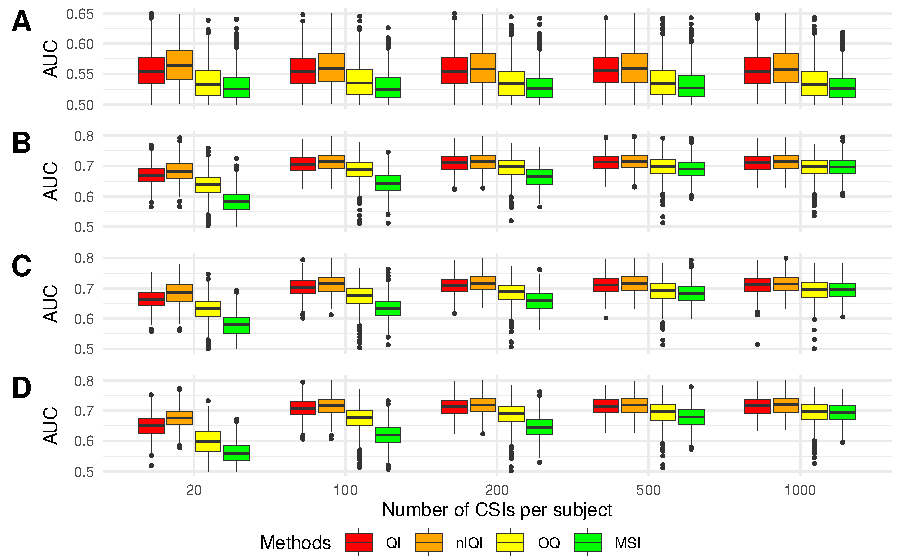
\includegraphics[height=2.7in] {Figures/Figures_simulations/AUC.box.plots nQ 19HRlabel2-3 pairedsimID 1000.pdf}
	\end{figure}  
}

% % % % % % % % % % % % % % % % % % % % % % % % % % % % % % % % % % % % %  	
\frame
   {\frametitle{AUC ROC estimates for High vs. Low risk group with HR=2-3 based on a large number of percentiles ($p=0.01, 0.02, \dots, 0.99$)}  
    	\begin{figure}
	  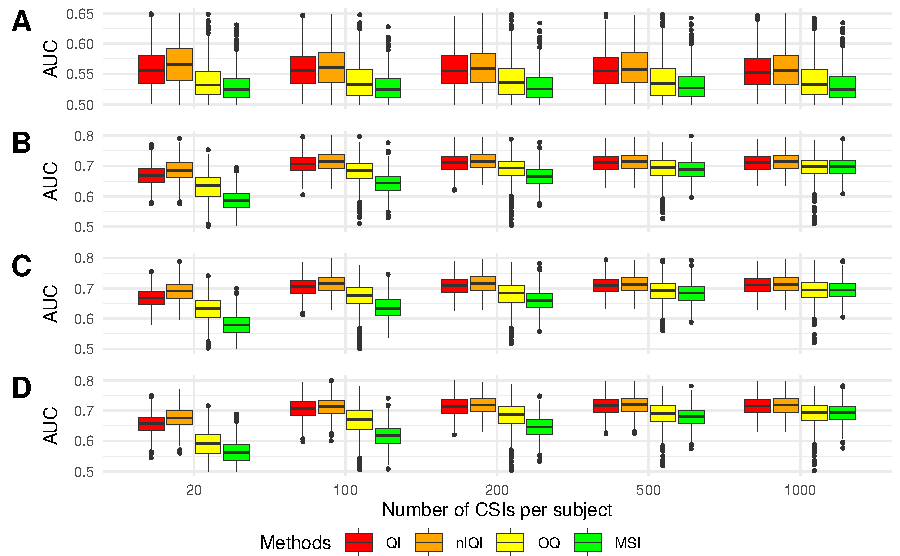
\includegraphics[height=2.7in] {Figures/Figures_simulations/AUC.box.plots nQ 99HRlabel2-3 pairedsimID 1000.pdf}
	\end{figure}  
}

% % % % % % % % % % % % % % % % % % % % % % % % % % % % % % % % % % % % %  	
\frame
   {\frametitle{Misclassification error for High vs. Low risk group with HR=2-3 based on a small number of percentiles ($p=0.05, 0.1, \dots, 0.95$)}  
    	\begin{figure}
	  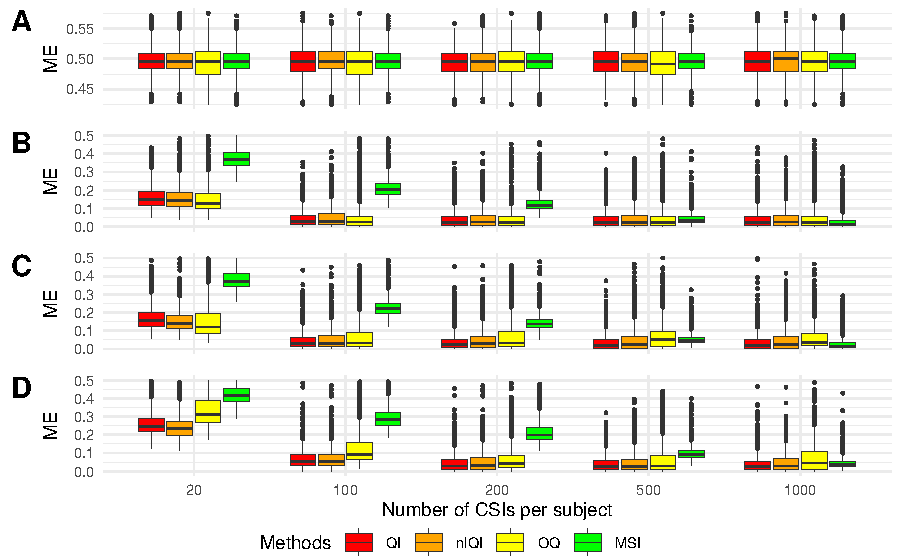
\includegraphics[height=2.7in] {Figures/Figures_simulations/ME.box.plots nQ 19HRlabel2-3 pairedsimID 1000.pdf}
	\end{figure}  
}

% % % % % % % % % % % % % % % % % % % % % % % % % % % % % % % % % % % % %  	
\frame
   {\frametitle{Misclassification error for High vs. Low risk group with HR=2-3 based on a large number of percentiles ($p=0.01, 0.02, \dots, 0.99$)}  
    	\begin{figure}
	  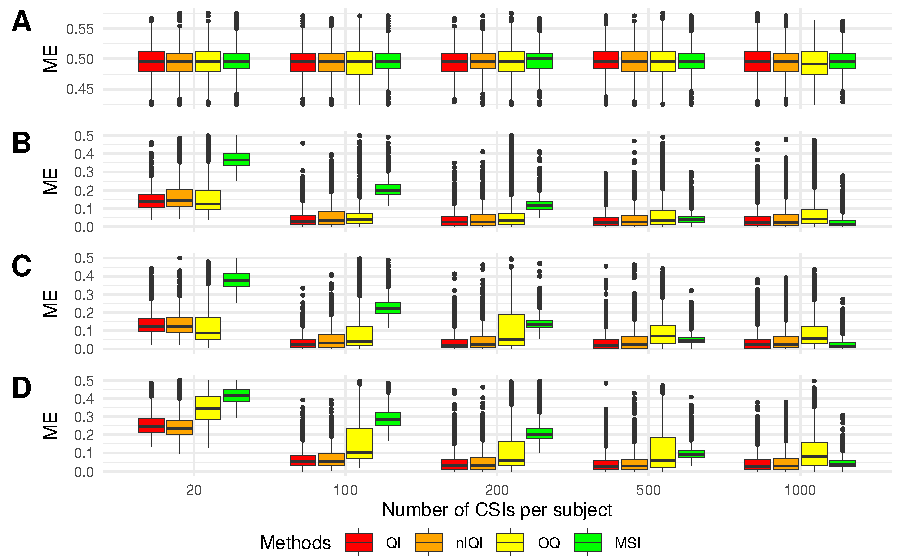
\includegraphics[height=2.7in] {Figures/Figures_simulations/ME.box.plots nQ 99HRlabel2-3 pairedsimID 1000.pdf}
	\end{figure}  
}


% % % % % % % % % % % % % % % % % % % % % % % % % % % % % % % % % % % % %  	
%\frame
%   {\frametitle{Conclusions from simulation studies}  
%}

% % % % % % % % % % % % % % % % % % % % % % % % % % % % % % % % % % % % %  concluding  
	\frame
	{\frametitle {Conclusions and future directions}  
	 \begin{itemize}
     \item Biomarkers based on entire distributions of CSI values of the protein of interest provide more information than the ones based on MSI or optimal quantiles.
     	\item Linear FR-QI and nonlinear nlFR-QI performed similarly in our simulation scenarios. 
	\item Performance was similar for FR-QI and nlFR-QI biomarkers based on a small ($p=0.05, 0.1, \dots, 0.95$) 
	 or a large ($p=0.01, 0.02, \dots, 0.99$) number of percentiles.
	 \item The level of separation of survival curves between high vs. low risk groups had limited effect on performance of FR-QI biomarkers.
	\item In data with moderate sample sizes, FR-QI tends to be more efficient than nlFR-QI.
		\item Interpretation of nlFR-QI biomarkers is potentially more challenging.
	\item Dichotomized versions of FR-QI biomarkers are more informative for some proteins, but continuous FR-QI biomarkers tend to be more reproducible in an external validation. 
	 \item For valid new biomarkers, it is necessary to validate FR-QI and nlFR-QI metrics in a test set. 
	 	\color{red}
	 	 \item Proposed  FR-QI and nlFR-QI are applicable to any technology that captures protein or gene expression levels in individual cells or cell compartments (e.g. flow cytometry)
	 	\color{blue}
	\item  Additional work is needed to address aggregation of information from multiple cores or regions of interest per subject. 
        \item  Linear and nonlinear functional regression indices can be derived using functional predictors other than CSI quantile functions.
          \end{itemize}  
	}

\begin{frame}
\frametitle{Acknowledgments}   

       \begin{columns}[T]
       
		      \begin{column}{0.2\textwidth}
			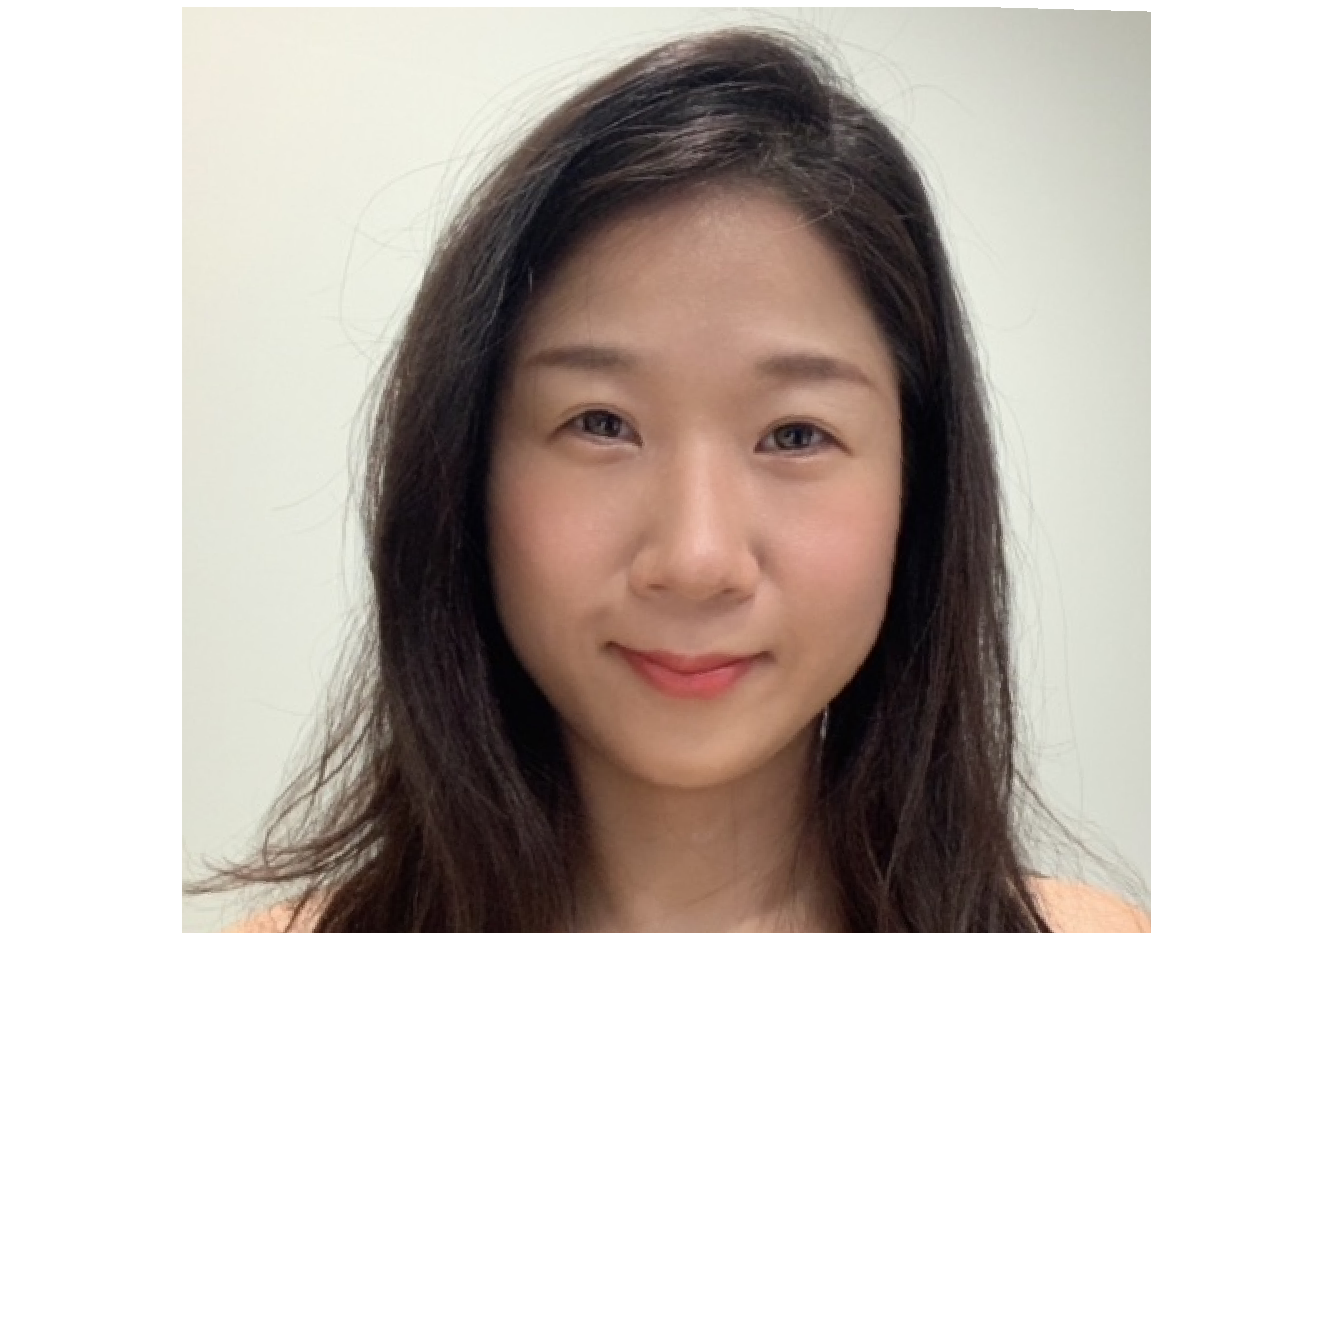
\includegraphics[height=0.8in] {Figures/Misung.pdf}
			   \caption{ \textbf{Misung Yi, \\PhD$^{1,3}$} }
		 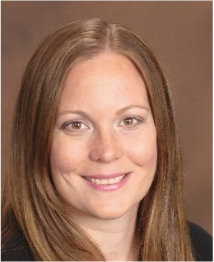
\includegraphics[height=1in] {Figures/Amy.png}
				   \caption{\textbf{Amy R. Peck, PhD$^{2,3}$}}   			   
			       \end{column}
			       
		  \begin{column}{0.2\textwidth}
			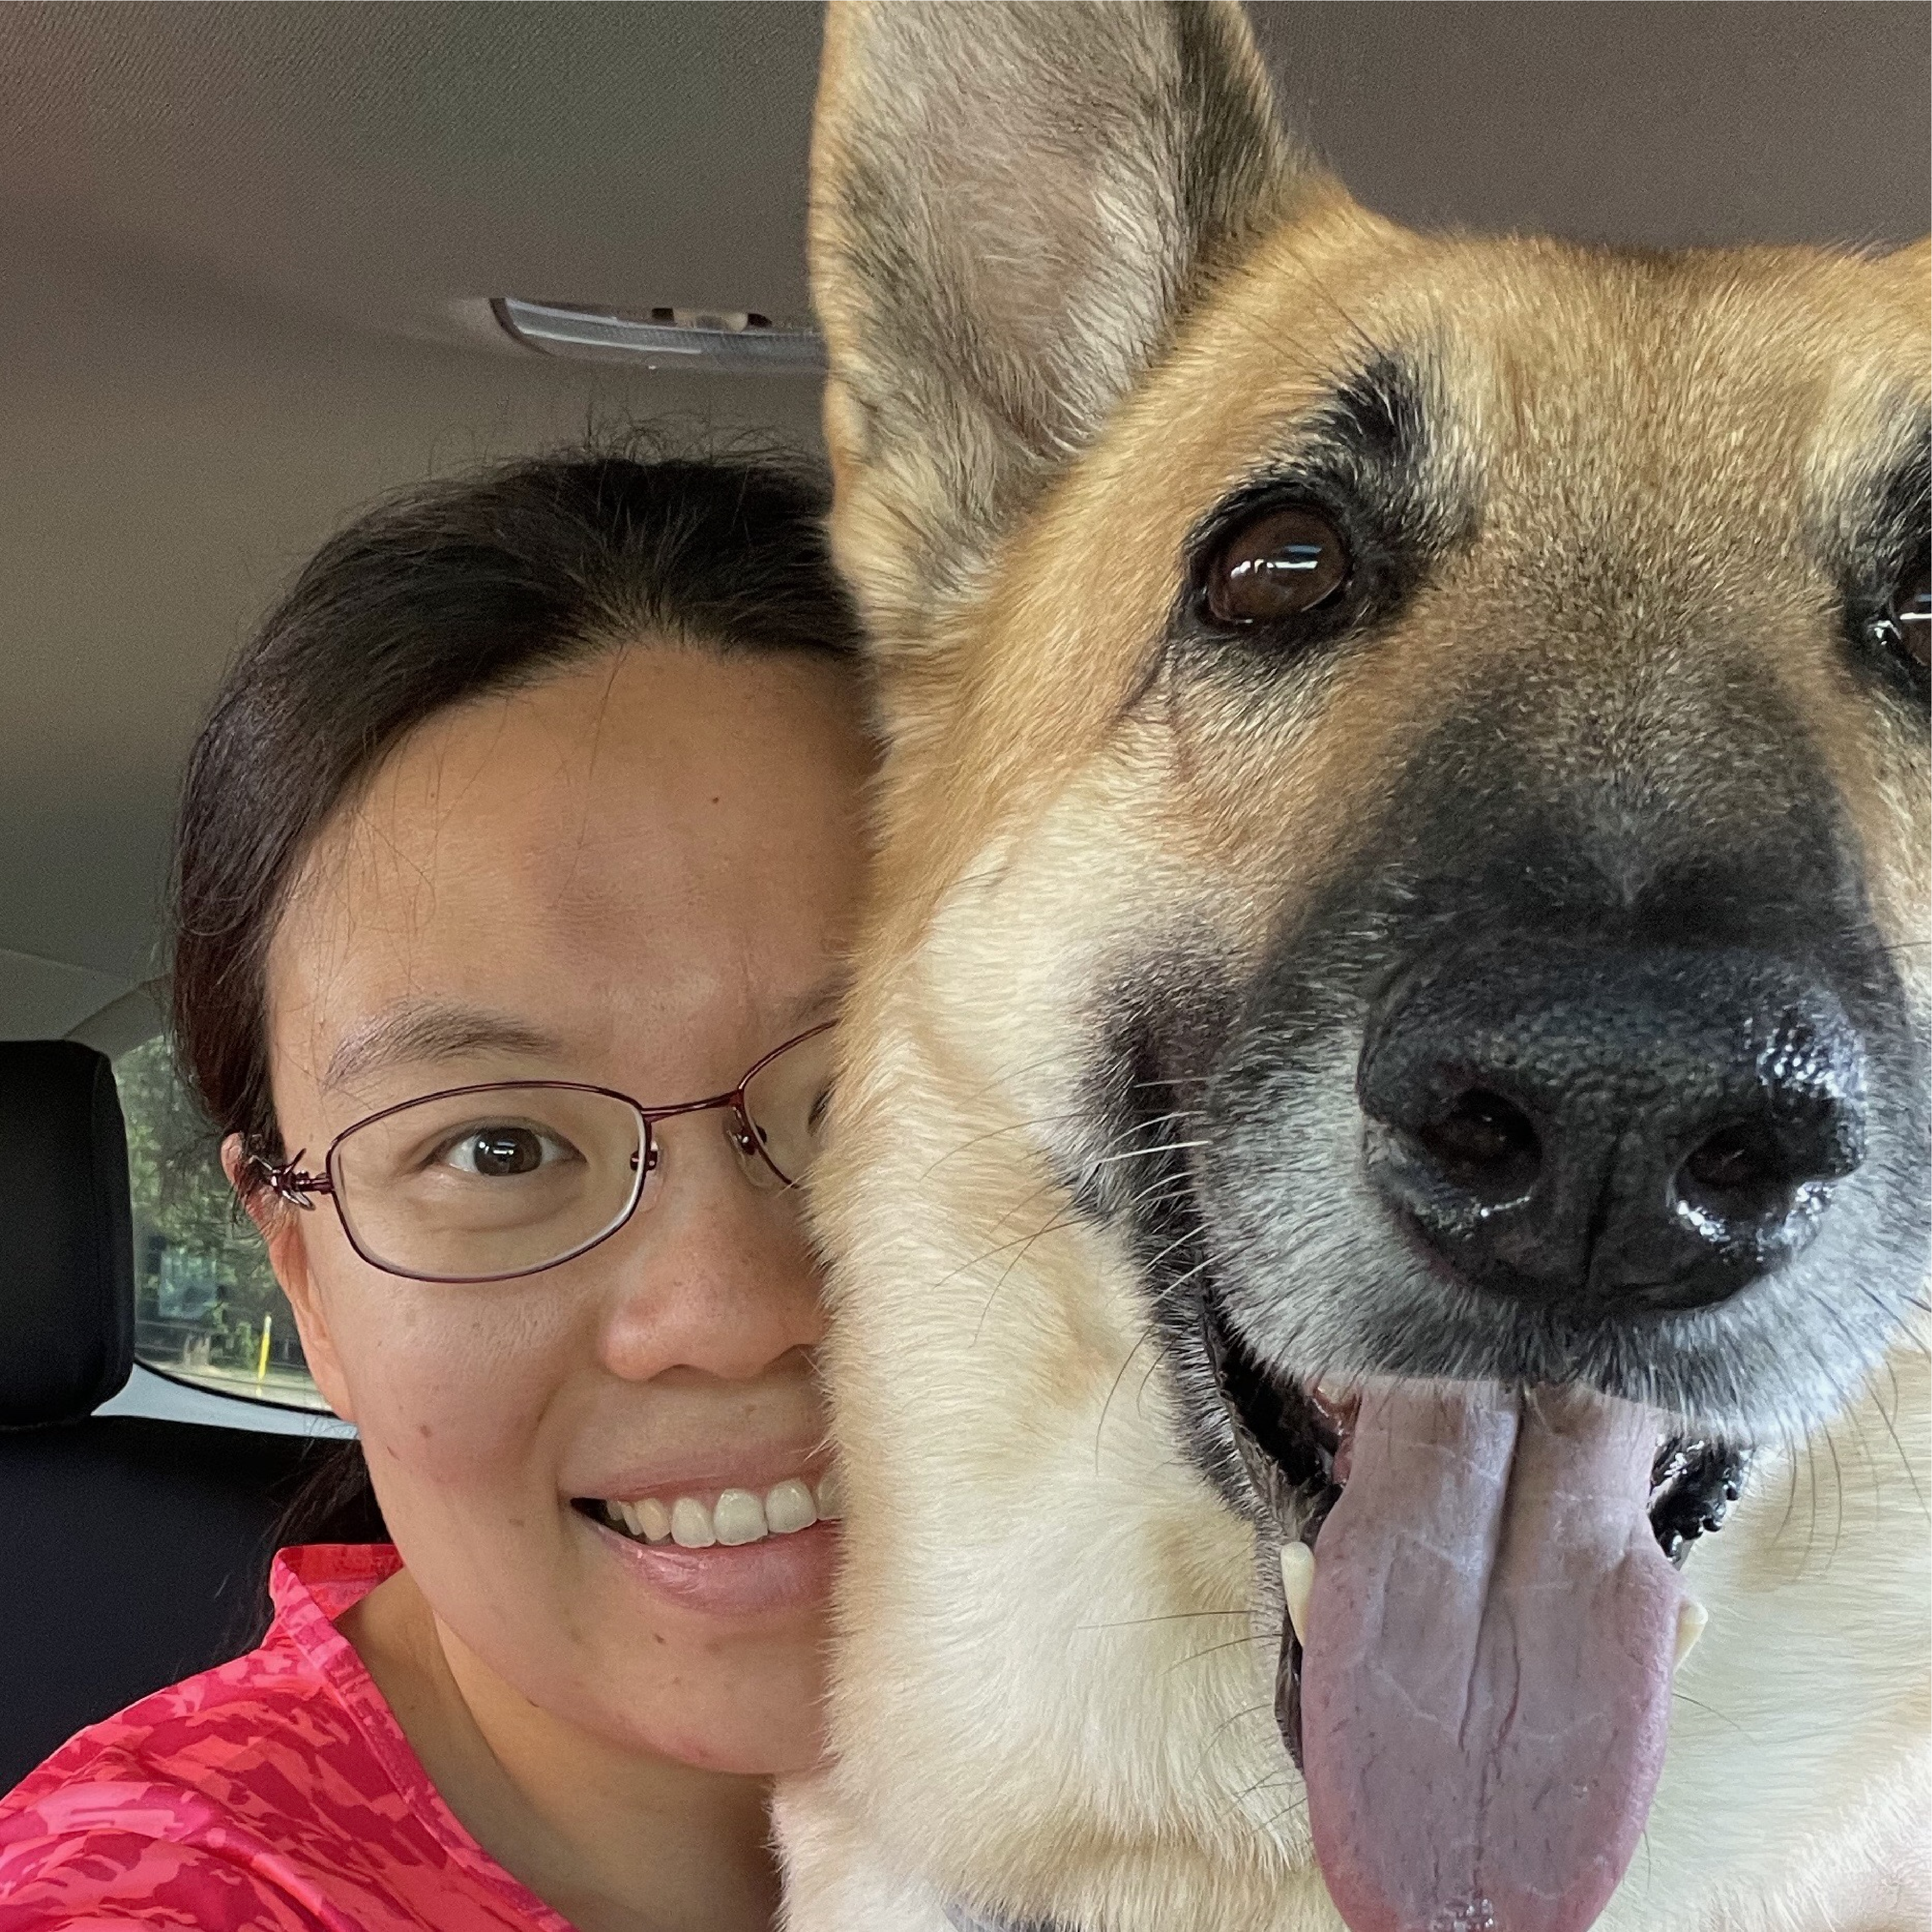
\includegraphics[height=0.8in] {Figures/Tingting.pdf}
			  \caption{\textbf{Tingting Zhan, PhD$^{1,3}$}}
	          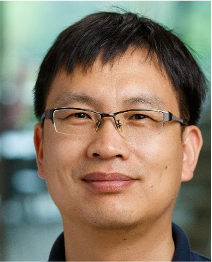
\includegraphics[height=1in] {Figures/Yunguang.png}
		       \caption{\textbf{Yunguang Sun, PhD$^4$}}	  			  
			       \end{column}	
			       	
	          \begin{column}{0.2\textwidth}
			
\includegraphics[height=0.8in] {Figures/Rui.png}
			  \caption{\textbf{Hallgeir Rui,\\MD, PhD$^{2,3}$}}
		 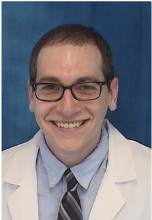
\includegraphics[height=1in] {Figures/Maisel.png}
		 \caption{\textbf{Brenton Maisel, MD, PhD$^5$}}
			       \end{column}	
		      
		      	  \begin{column}{0.4\textwidth}
	             \textbf{Funding:}\\
                      
\includegraphics[height=0.3in] {Figures/Komen.png}\\
Promise grant \textit{Therapy-relevant stratification of breast cancer patients:  Integrating pathology and biomarker analyses} (PI: Rui)\\
\bigskip
			 
\includegraphics[height=0.3in] {Figures/NCI.jpeg}\\
		 \color{red}
			  NIH/NCI R01 CA222847\\
			(PI: Chervoneva)\\	
			\color{black}
		  NIH/NCI R01 CA267549\\
		 (MPIs: Rui, Chervoneva)\\
		      \end{column}	
	\end{columns}	
 $^{1}$ Division of Biostatistics,   $^{2}$ Division of Cancer Biology, 
 $^{3}$ Department of Pharmacology, Physiology and Cancer Biology,  Sidney Kimmel Medical College, Thomas Jefferson University\\
 $^{4}$ Department of Pathology, Medical College of Wisconsin\\
  $^{5}$ Department of Neurology, University of California Irvine
\end{frame}	
	% % % % % % % % % % % % % % % % % % % % % % % % % % % % % % % % % % % % % 
	\frame
	{\frametitle { }  
		\begin{figure}
			
\includegraphics[height=0.5in] {Figures/Thank_you.pdf}
		\end{figure} 
\begin{center}		
\begin{huge}		
Any questions? \\
Please contact me at \\
\\
Inna.Chervoneva@jefferson.edu
\end{huge}	
\end{center}
\bigskip		
		\begin{figure}
     
\includegraphics[height=1in] {Figures/Ukr_flag.jpeg}
           %  
\includegraphics[height=1.5in] {Figures/SU.png}
\end{figure} 
	}  
	

	
\end{document}






